% compile with
%   xelatex --shel-escape p01-introducao
% or
%   latexmk -pvc -pdf -pdflatex=xelatex -latexoption=--shell-escape p01-introducao
%

\documentclass[11pt,fleqn]{practice}

\usepackage{siunitx}

\begin{document}

\tcbset{lowerbox=ignored}

\institution{UFOP\quad DECOM}
\course{Programação de Computadores I}
\subtitle{Aula prática 1}
\title{O Ambiente Scilab}
\author{José Romildo Malaquias\thanks{\url{romildo@iceb.ufop.br}}}
\date{2014--2}
\maketitle

\begin{abstract}
  Nesta aula o aluno deverá se familiarizar com o ambiente de
  programação do Scilab através da avaliação de expressões na janela do
  console, e da edição e execução de arquivos de programa.
\end{abstract}

\tableofcontents

\section{Páginas importantes para a disciplina}

Antes de iniciar as atividades de programação, realize as tarefas
seguintes para cadastro nas páginas da disciplina.

\begin{task}{Site da disciplina}{}
  Visite o site da disciplina para as turmas 17 e 18 em
  \url{http://www.decom.ufop.br/romildo/2014-1/bcc701/} e leia
  rapidamente as informações sobre a disciplina.

  Visite também o site geral da disciplina em
  \url{http://www.decom.ufop.br/bcc701}.
\end{task}

\begin{task}{Grupo de discussão}{}
  \textbf{\textit{Atividade para casa.}} Visite o site do grupo de
  discussão da disciplina \url{http://groups.google.com/group/bcc701} e
  se cadastre no mesmo, para que você fique atualizado sobre o andamento
  da disciplina e possa participar das discussões pertinentes à
  disciplina.

  O grupo poderá ser usado para comunicação entre os
  participantes. Avisos poderão ser postados. Quando você tiver uma
  dúvida sobre o conteúdo da disciplina, você poderá expô-la no
  grupo. Assim outros participantes, incluindo os colegas, os
  professores e os monitores, poderão contribuir para o esclarecimento
  da dúvida. Outros alunos que porventura compartilham a mesma dúvida
  também estarão sendo beneficiados.
\end{task}

\begin{task}{Moodle}{}
  Visite o site da plataforma moodle do DECOM
  \url{http://www.decom.ufop.br/moodle/course/view.php?id=316} e se
  cadastre na mesma. Em seguida se inscreva no curso desta disciplina.

  A plataforma moodle será usada para submissão das soluções das tarefas
  que serão propostas nesta aula, e também nas demais aulas práticas.

  Os arquivos solicitados em uma aula prática deverão ser agrupados no
  formato \emph{zip} ou \emph{rar} usando ferramentas como
  \textbf{p7zip} ou \textbf{WinRar}, e o arquivo produzido deverá ser
  submetido.
\end{task}

\begin{task}{Site do Scilab}{}
  \textbf{\textit{Atividade para casa.}} Visite o site do Scilab em
  \url{http://www.scilab.org/}, onde você poderá encontrar várias
  informações sobre o ambiente Scilab.

  Se você desejar instalar o Scilab em um computador, faça o download do
  programa de instalação para a plataforma desejada (Linux, Windows ou
  Mac OS X) visitando a página
  \url{http://www.scilab.org/download/5.4.1}, e depois execute-o para
  instalar o Scilab.
\end{task}

\section{Avaliação de expressões}

O Scilab permite avaliar expressões diretamente na janela do
console. Nas tarefas que se seguem você deverá usar o console para obter
o valor de algumas expressões.

\subsection{Diário}

Porém antes de começar a calcular o valor das expressões, vamos aprender
a gravar em arquivo toda a sua atividade no console, de forma que você
(ou outras pessoas) possam revisar o que foi feito. Ao registro dos
comandos digitados no console, e suas respostas, chamamos de
\textbf{diário}.

Scilab permite que os comandos digitados no console durante uma sessão
sejam gravados em um arquivo texto, construindo uma espécie de
\emph{memória de cálculos}. O registro dos comandos é habilitado através
da utilizaçãoo da função \texttt{diary}:
\texttt{diary(\textsl{nome\_do\_arquivo})}.

Use a expressão \texttt{diary(\textsl{nome\_do\_arquivo})} para começar
a gravar um diário da sessão que ocorre no console. Uma cópia de todos
os dados de entrada digitados no console, e da maioria dos dados de
saída, é gravada no arquivo especificado. No lugar de
\texttt{\textsl{nome\_do\_arquivo}} você deverá usar o nome de arquivo
de sua preferência. Será criado um arquivo texto com este nome. Por
exemplo, após o comando \texttt{diary(tarefa1.txt)} será criado um
arquivo texto chamado \texttt{tarefa1.txt} e os próximos comandos e suas
respostas serão gravados neste arquivo.

A expressão \texttt{diary(\textsl{nome\_do\_arquivo}, 'close')} pode ser
usada para encerrar a gravação da sessão em arquivo de diário. Ao final
do registro da sessão este comando deve ser usado para fechar o diário.

Para suspender ou retomar a gravação da sessão em arquivo de diário você
pode ser as respectivas expressões
\texttt{diary(\textsl{nome\_do\_arquivo}, 'pause')} e
\texttt{diary(\textsl{nome\_do\_arquivo}, 'resume')}.

Como resultado das tarefas seguintes você deverá submeter um diário de
sessão de sua iteração com o console do Scilab para efetuar os cálculos
solicitados.


\subsection{Dicas}

Algumas \textbf{dicas} sobre a avaliação de expressões matemáticas no
Scilab:
\begin{itemize}
  \item Números decimais devem usar o ponto (\texttt{.}), e não a
  vírgula (\texttt{,}), para separar a parte inteira da parte
  fracionária. Assim o número 12,568 deve ser inserido como 12.568.

  \item Alguma constantes já estão disponíveis no Scilab na forma de
  variáveis predefinidas. Algumas delas são:

  \begin{tabularx}{\linewidth}{|l|X|}\hline
    \textbf{variável predefinia} & \textbf{valor} \\\hline
    \texttt{\%pi} & aproximação do número irracional $\pi = 3.1415927...$ \\\hline
    \texttt{\%e}  & aproximação do número irracional $e = 2.7182818...$\newline (número neperiano) \\\hline
    \texttt{\%i}  & unidade imaginária $i$ \\\hline
  \end{tabularx}

  \item O Scilab oferece várias funções predefinidas. Algumas delas são:

  \begin{tabular}{|l|l|}\hline
    \textbf{função predefinia} & \textbf{descrição} \\\hline
    \texttt{abs}   & valor absoluto \\\hline
    \texttt{sqrt}  & raiz quadrada (\emph{square root}) \\\hline
    \texttt{sin}   & seno \\\hline
    \texttt{cos}   & cosseno \\\hline
    \texttt{tan}   & tangente \\\hline
    \texttt{log}   & logaritmo natural (base $e$) \\\hline
    \texttt{log10} & logaritmo decimal (base 10) \\\hline
  \end{tabular}

  \item O operador de multiplicação \texttt{*} sempre deve ser escrito
  explicitamente para realizar uma multiplicação.

  Por exemplo, para calcular a área $A$ de um círculo de raio $r =
  2,5m$, dada por \[ A = \pi r^2 \] usamos
  \begin{lst}{scilab}
--> r = 2.5
 r  =
 
    2.5  
 
--> A = %pi * r^2
 A  =
 
    19.634954
  \end{lst}

  \item Aplicações de função devem sempre ser escritas colocando o(s)
  argumento(s) da função entre parênteses, logo depois do nome da
  função. Esta regra deve ser observada mesmo quando a notação
  matemática dispensa o uso de parênteses. Evite deixar espaços entre o
  nome da função e o parêntese.

  Por exemplo, para calcular o valor da expressão \[\sin{(3\pi)} -
  \cos{0} + \log_{10}{1000} \] fazemos
  \begin{lst}{scilab}
--> sin(3 * %pi) - cos(0) + log10(1000)
 ans  =
 
    2.  
  \end{lst}

  \item O cálculo da raiz quadrada pode ser feito usando tanto a função
  predefinida \texttt{sqrt} quanto a operação de potenciação com
  expoente $\frac{1}{2}$.

  A radiciação com índice diferente de 2 pode ser feita por meio de uma
  potenciação usando expoente fracionário, de acordo com a propriedade

  \[ \sqrt[n]{x} = x ^ \frac{1}{n} \]

  \item Sempre que necessário use parênteses para agrupar subexpressões
  que aparecem em expressões maiores, observando as regras de prioridade
  dos operadores. Lembre-se que entre os operadores aritméticos, a
  potenciação (\texttt{\textasciicircum}) tem maior prioridade, seguida
  da multiplicação (\texttt{*}) e divisão (\texttt{/}), seguidas da
  adição (\texttt{+}) e subtração (\texttt{-}), como é usual na notação
  matemática.

  Por exemplo, para avaliar a expressão \[ \frac{2}{\sqrt{a} - b^2} +
  a^{2b} \] onde $a = 3$ e $b = 5$, fazemos
  \begin{lst}{scilab}
-->a = 3
 a  =
 
    3.  
 
-->b = 5
 b  =
 
    5.  
 
-->2/(sqrt(a) - b^2) + a^(2*b)
 ans  =
 
    59048.914
  \end{lst}
  Observe que o denominador da fração precisou ser escrito entre
  parênteses, pois a subtração tem prioridade menor que a divisão. De
  maneira semelhante, o expoente da última potenciação precisou ficar
  entre parênteses, já que a multiplicação tem menor prioridade que a
  potenciação.

  \item Ao escrever uma expressão para calcular alguma grandeza física,
  deve-se digitar apenas o seu valor, sem incluir a unidade de
  medida. Os valores das grandezas já devem estar consistentes com o
  sistema de unidades usado.

  Por exemplo, para calcular a distância percorrida por um veículo que
  viaja a uma velocidade média de \SI{110,8}{km/h} no intervalo de tempo
  de \SI{90}{min}, é necessário converter o tempo (que está em minutos)
  para horas, já que a velocidade foi dada em \si{km/h}. O resultado
  será obtido em \si{km}. O cálculo é feito usando a equação
  \[ v_m = \frac{\Delta s}{\Delta t} \]
  onde $v_m$ é a velocidade média, $\Delta s$ é a distância percorrida,
  e $\Delta t$ é o tempo gasto em percorrê-la. Desta equação obtém-se
  \[ \Delta s = v_m \Delta t \]
  \begin{lst}{scilab}
--> vm = 110.8
 vm  =
 
    110.8  
 
--> dt = 90/60
 dt  =
 
    1.5  
 
--> ds = vm * dt
 ds  =
 
    166.2  
  \end{lst}
\end{itemize}

\subsection{Avaliando expressões}

Nas tarefas seguintes você deverá submeter o \emph{arquivo de diário}
solicitado em cada tarefa.

\begin{task}[breakable,fontlower=\small]{Movimento Retilínio Uniformementne Variado}{}
  A posição $s$ de um corpo em movimento retilínio uniformemente
  variado, em função do tempo $t$, é dado pela equação
  \[ s = s_0 + v_0 t + \frac{1}{2} a t^2 \]
  onde $x_0$ é a posição inicial do corpo, $v_0$ é a sua velocidade
  inicial, e $a$ é a acelaração.

  Utilize o console do Scilab para calcular a posição de uma bola em
  queda livre no instante $t = \SI{8}{s}$, considerando que a posição
  inicial é $s_0 = \SI{100}{m}$, a velocidade inicial é $v_0 =
  \SI{15}{m/s}$ e a acelaração da gravidade é $a = \SI{-9,81}{m/s^2}$.

  Você deverá registrar a sua sessão no console em um arquivo de diário
  chamado \texttt{quedalivre.txt}.

  \tcblower
  \solution
  \begin{lst}{scilab}
-->diary("quedalivre.txt");
 
-->s0 = 10;
 
-->v0 = 15;
 
-->a = -9.81;
  
-->t = 5;
 
-->s = s0 + v0*t + 1/2*a*t^2
 s  =
 
  - 37.625  
 
-->diary("quedalivre.txt", 'close');
  \end{lst}
\end{task}

\begin{task}[breakable,fontlower=\small]{Expressões matemáticas}{}
  Utilize o Scilab para avaliar as expressões aritméticas seguintes,
  considerando que $x = 3$ e $y = 4$.

  Você deverá registrar a sua sessão no console em um arquivo de diário
  chamado \texttt{calculos.txt}.

  \begin{enumerate}
    \item $\displaystyle \frac{4}{3}\pi \sin{x^2 - 1} $
    \item $\displaystyle \frac{x^2 y^3}{(x - y)^2} $
    \item $\displaystyle \frac{1}{x^2 - y} - e^{-4x} +
    \sqrt[3]{\frac{35}{y}} \sqrt{xy} $
    \item $\displaystyle \frac{24 + 4.5^3}{e^{4.4} - log_{10}{12560}} $
    \item $\displaystyle \cos{\frac{5\pi}{6}} \sin^2{\frac{7\pi}{8}} +
    \frac{\tan{(\frac{\pi}{6}\ln{8})}}{\sqrt{7}+2} $
  \end{enumerate}

  \tcblower
  \solution
  \begin{lst}{scilab}
-->diary("calculos.txt");
 
-->x = 3;
 
-->y = 4;
 
-->4/3 * %pi * sin(x^2) - 1
 ans  =
 
    0.7262779  
 
-->x^2 * y^3 / (x-y)^2
 ans  =
 
    576.  
 
-->1/(x^2-y) - %e^(-4*x) + (35/y)^(1/3)*(x*y)^(1/2)
 ans  =
 
    7.3382694  
 
-->(24 + 4.5^3)/(%e^4.4 - log10(12560))
 ans  =
 
    1.4883284  
 
-->cos(5*%pi/6)*(sin(7*%pi/8))^2 + tan(%pi/6*log(8))/(sqrt(7)+2)
 ans  =
 
    0.2846166  
 
-->diary("calculos.txt", 'close');
  \end{lst}
\end{task}

\section{Edição de programas}

Nas tarefas seguintes você deverá submeter o \emph{arquivo de programa}
solicitado, e também um \emph{arquivo de imagem} do gráfico produzido
pela execução do programa.

O menu da janela de gráficos disponibiliza um comando que permite gravar
o gráfico em arquivo.

\begin{task}{Gráfico da função $f(x) = 2e^{-0.2x}$}{}
  As seguintes declarações Scilab desenham a função \[f(x) =
  2e^{-0.2x}\] no intervalo $0 \le x \le 10$.

  \begin{lst}{scilab}
x = 0 : 0.1 : 10;
y = 2 * exp(-0.2 * x);
plot(x, y);
  \end{lst}

  Utilize a janela de edição do Scilab para criar um novo arquivo de
  programa, digite essas declarações no arquivo e grave o arquivo com o
  nome \texttt{teste1.sce}.

  Em seguida execute o programa usando o menu \textit{Execute -> Save
    and Execute}, ou a tecla \texttt{F5}, ou ainda o botão \textit{Save
    and Execute} da barra de tarefas do SciNotes. Que resultado você
  obtém?

  \tcblower
  \solution
  O gráfico da função dada é desenhado na janela de gráficos:
  \begin{center}
    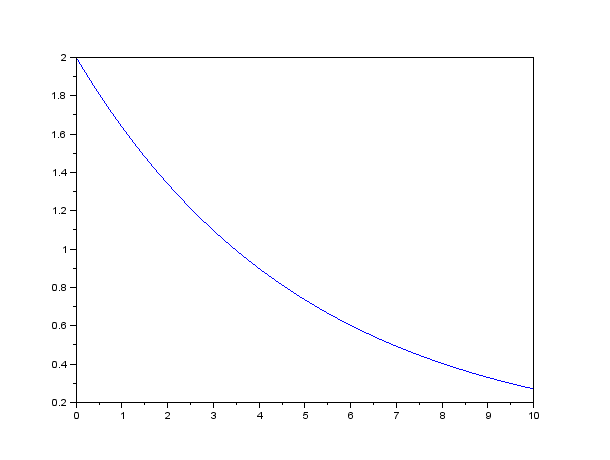
\includegraphics[width=\linewidth]{images/grafico1}
  \end{center}
\end{task}

\begin{task}{Gráfico da função $f(x) = |sin x|$}{}
  Usando os comandos disponíveis no menu no ambiente Scilab, mude o
  diretório (pasta) atual para um novo diretório chamado
  \texttt{MeusProgramas} e edite o arquivo de programa
  \texttt{teste2.sce} neste diretório usando o SciNotes.

  O conteúdo do novo arquivo deve ser
  \begin{lst}{scilab}
// Cria um vetor correspondente ao intervalo de -2*%pi até 2*%pi
t = -2*%pi : %pi/10 : 2*%pi;

// Calcula |sin(t)|
x = abs(sin(t));

// Plota o resultado
plot(t, x);
  \end{lst}

  Execute o programa. O que acontece?

  \tcblower
  \solution
  O gráfico da função dada é desenhado na janela de gráficos:
  \begin{center}
    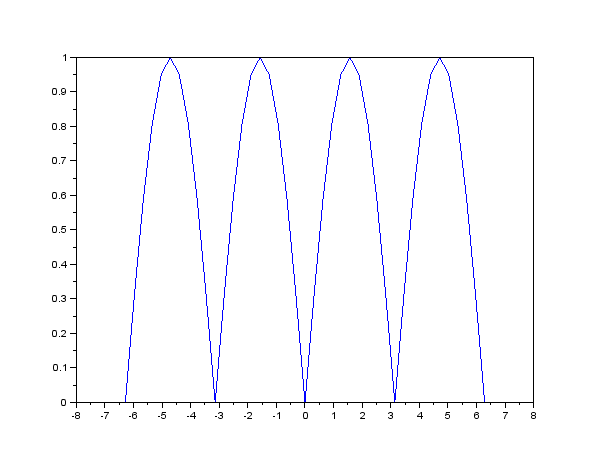
\includegraphics[width=\linewidth]{images/grafico2}
  \end{center}
\end{task}


\end{document}
